\section{Cloud System Models}\label{sec:cloud-models}
\noindent Current cloud systems do not ignore SLA restrictions; rather, they are designed from the ground up to support a single type of SLA.  That SLA generally encompasses total system uptime and some kind of response time metric \cite{ctrl:amazon-sla,ctrl:rackspace-sla}.  If for some reason the cloud provider can no longer adhere to the terms outlined, some kind of compensation strategy generally applies to affected customers.  Future cloud providers can very well use the ability to support multiple SLAs as a way to differentiate available products from competitors.

\begin{figure}[!t]
\centering
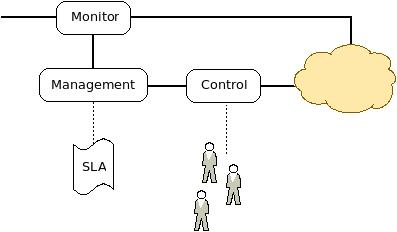
\includegraphics[width=3in]{cloud-current}
\caption{Single SLA with Control Elements}
\label{fig:current-cloud-model}
\end{figure}

\subsection{Current Model}
Current systems like Amazon's EC2 or Rackspace products are designed around high availability, and this is reflected in the focus of their supplied SLAs.  This common design focus is also evident in the artifacts generated by other vendors \cite{ctrl:google-arch}.  Furthermore, Amazon offers clear guidance on how to develop systems that take advantage of their robust architecture as well as services that provide some measure of automatic scaling \cite{ctrl:amazon-best-practice,ctrl:amazon-fault-tolerant}.  This combination of market leading position and products and the extensive supplied guidance make Amazon a clear choice to examine when reflecting on the current state-of-the-art.

Amazon's Cloud Watch products used in tandem with Auto Scaling provide the ability to control the number of deployed instances in response to specific system loads, as shown in Figure \ref{fig:current-cloud-model} \cite{ctrl:amazon-cloud-watch,ctrl:amazon-auto-scale}.  Cloud Watch gives customers the ability to monitor various system performance metrics for their virtual machines, including but not limited to latency, processor use, and request counts.  Furthermore, users can set resource levels at which additional EC2 instances are created or destroyed.  This provides some level of personalized management and control over deployed systems within Amazon's cloud infrastructure.

\subsection{Future Reference Model}
While current cloud service providers focus on a single QoS metric, future providers may very well begin to provide multiple metrics over which they will define service levels, as shown in Figure \ref{fig:future-cloud-model}.  This is not without precedent --- just as airlines provide the same essential product at different service points, cloud providers could supply system hosting via disparate service levels, including divergent service metric definitions.  For example, current architectures support uptime and availability as the primary managed metric from an SLA perspective.  Future architectures could support uptime and availability, as well as specific latency, bandwidth, and geo-location sensitive hosting parameters.  These kinds of SLAs would also continue to outline penalties when any of the conditions of that SLA were violated.  Unlike current SLAs however, these could also differentiate based on the magnitude of the imposed penalty, with different classifications of service mapping to increasingly large penalties on service failure.

\begin{figure}[!t]
\centering
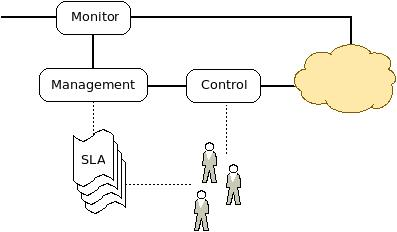
\includegraphics[width=3in]{cloud-future}
\caption{Multiple SLA Architectural Integration}
\label{fig:future-cloud-model}
\end{figure}

While industry does seem to certainly be trending in this direction, as indicated by the development of tools supporting user-centric infrastructure monitoring and management, this kind of control is not yet embedded into contracts of any kind, much less agreements that are machine-readable. Furthermore, this kind of management is still manual and cannot scale to the levels needed to manage Internet-scale systems.

\section{Service Level Agreements Defined}\label{sec:SLA-defined}
As we have seen, SLAs generally consist of a set of conditions of use under which the SLA is binding, a set of obligations that the provider will adhere to if the customer adheres to the set conditions, and two sets of penalties, one penalizing the provider when breaching obligations, and another penalizing the customer when breaching conditions of use.  Conditions are generally loosely defined, while provider obligations are much more rigorously constructed.  Generally however, conditions and obligations in this context can be viewed as defined by {\it objectives} which are measured by {\it indicators}.  In the case of provider-centric obligations, these are commonly defined as service level indicators (SLIs) and objectives (SLOs).

With this general understanding of SLAs and related SLIs and SLOs, we can create a non-specific definition of an SLA as a set of tuples:
\begin{equation}
SLA = \lbrace (I,O,E,P)_{0..n} \rbrace, n \in Z \\
\end{equation}
Where $ I $ is an indicator function, $ \forall i \in I, i : () \rightarrow \tau $, which retrieve indicator values, generally related to some kind of SLI or customer condition indicator.  Parameter $ O $ is a set of values derived from SLOs or customer condition objectives such that $ \forall o \in O, o : P(\tau) $.  Parameter $ E $ is a set of predicates that indicate whether a specific indicator complies with its objectives, where $ \forall e \in E, e : ( () \rightarrow \tau ) \times P(\tau) \rightarrow bool $.  Parameter $ P $ is a set of penalty functions, $ \forall p \in P, p : Z \rightarrow Z $, where the first argument is generally an elapsed time value.

For example, say we are a customer of Nimbus Cloud Corporation, and we have an SLA in which Nimbus provides guaranteed 100\% uptime and packet latency between 300 and 650 milliseconds.  Nimbus does not have any customer conditions specified within its SLAs.  This then gives us a machine evaluateable SLA:
\begin{align}
SLA_{nimbus} = ( ( uptime\_monitor() : bool, \notag\\
\lbrace true \rbrace, \notag \\
uptime\_evaluator( monitor : () \rightarrow bool, \lbrace true \rbrace) : bool, \notag \\
uptime\_penalty\_evaluator( T : Z ) : Z ), \notag \\
( latency\_monitor() : Z, \notag \\
\lbrace 300, 650 \rbrace, \notag \\
latency\_evaluator( monitor : () \rightarrow Z, \lbrace 300, 650 \rbrace) : bool, \notag \\
latency\_penalty\_evaluator( T : Z ) : Z) ) \notag
\end{align}
This more rigorous SLA allows users to monitor obligations and determine penalties when triggered.

\section{Evaluating and Verifying Service Level Agreements}\label{sec:SLA-analysis}
Now that we have rigorously defined our SLAs, notice that the SLA evaluation functions are predicates, and can be curried for later execution if needed.  This allows us to begin a more fundamental analysis of SLAs and their capabilities.

\subsection{Computational and Space Complexity}
In Section \ref{sec:SLA-defined}, we defined an SLA to essentially be a sequence of evaluatable predicates.  These evaluatable predicates are related in some way; currently, an SLA is the conjunction of these predicates.  As these predicates can be created prior to evaluation, and at evaluation time require no specific arguments once appropriately curried, we can define these predicates as boolean {\it terms}.  Ergo, once we have created a group of predicates and transformed them into terms, we are evaluating an arbitrary boolean equation - in other words, we are verifying an instance of the Boolean Satisfiability Problem, or SAT.\\

\noindent {\bf Claim 1:} SLA is in {\bf NP}.\\

\noindent {\bf Proof:} The following verifier runs in polynomial time in the length of an SLA.\\

\begin{tabbing}
\noindent Veri\=fier\=~$V \langle SLA \rangle$ : \\
\> \underline{for} each clause $ c \in SLA $ :\\
\>\> extract monitor $ m \in M $ from $ c $\\
\>\> extract objective $ o \in O $ from $ c $\\
\>\> extract evaluator $ e \in E $ from $ c $\\
\>\> $ r \leftarrow e ( m, o ) $\\
\>\> \underline{if} $ r = false $ \underline{return} false\\
\> \underline{return} true\\
\end{tabbing}

\noindent We can furthermore establish that SLA-SAT is NP-Hard.\\

\noindent {\bf Claim 2:} SAT $ \leq_{p} $ SLA-SAT.\\

\noindent {\bf Proof:} ADD PROOF \\

$ SAT $ is NP-Complete, and provably difficult to solve \cite{comptheory:sipser:intro-comp-theory}.  $ 3SAT $, a subset of $ SAT $, is equally difficult, while $ 2SAT $ is not.  $ 2SAT $ is firmly in the computational class $ P $; in fact, $ 2SAT $ is NL-Complete as well, so we know it is solvable in an amount of space logarithmic in the number of boolean terms \cite{comptheory:papadimitriou:computational-complexity}; it is widely believed that both $ SAT $ and $ 3SAT $ cannot be solved in logarithmic or less space.  Finally, as $ 2SAT $ is NL-Complete, we also know it is contained within NC$^{2}$, and as such is highly parallelizeable \cite{comptheory:papadimitriou:computational-complexity}.

\subsection{Verification v. Solution}
General SLA use focuses on verification rather than solution.  That is to say, with respect to a given SLA, both the user and provider is more concerned with whether the system is currently compliant with all SLA terms.  In future use, this may very well no longer be the case.  For example, imagine a cloud system from the user's perspective that spans multiple cloud providers; a single general purpose provider for general computing, data storage, and queuing, a specific-use provider for an unique set of algorithms of some kind (say, market modeling algorithms), and finally a Content Delivery Network (CDN) provider.  Each of these providers have a unique SLA with multiple conditions.  In this particular case, the user may need to know if the given system can work together at all under the terms of the SLAs, and if so, under what conditions.  As the user has combined all the SLAs composing the system and is attempting to find some combination of terms that satisfies the resulting boolean formula, the user is in essence attempting to find a solution for this instance of $ SAT $, a known NP-Complete problem.  Likewise, a cloud provider may need to solve similar problems where the SLAs at issue are the whole of SLAs issued to the entire provider's customer base.

Nontrivial generalized SLAs may be too difficult to solve effectively without using some kind of approximate heuristic or $ SAT $ Solver \cite{Hochbaum:1996:AAN:241938,ctrl:satcompetition}.  If these SLAs are formulated in at most a $ 2SAT $ style problem however, they are suddenly much more tractable, easier to work with, and amenable to efficient solution.  Keep in mind, even generalized SLAs can be efficiently verified.
